\documentclass[sigconf,authorversion,nonacm]{acmart}

\usepackage{minted}
\usemintedstyle{borland}
\setminted{linenos=true}

\usepackage{fontspec}
\setmonofont{Fira Code Retina}[Scale=MatchLowercase]

\captionsetup{justification=centering,margin=1cm}

\AtBeginDocument{%
  \providecommand\BibTeX{{%
    \normalfont B\kern-0.5em{\scshape i\kern-0.25em b}\kern-0.8em\TeX}}}

\begin{document}

\title{Tarea 3 \\ Optimización de enjambre de partículas}

\author{Mario Emilio Jiménez Vizcaíno}
\email{A01173359@itesm.mx}

\maketitle

\section{Introducción}
El algoritmo de optimización de enjambre de partículas es un algoritmo basado en las técnicas de cómputo evolutivo, primera vez descrito en 1995 por Kennedy y Eberhart \cite{kennedy1995particle}. La intención original era simular gráficamente el vuelo de una parvada de pájaros, y durante la evolución del algoritmo surgió el objetivo de utilizarlo como un algoritmo optimizador para funciones continuas no lineales.

Durante la ejecución de este algoritmo un número de entidades, las partículas, se colocan en el espacio de búsqueda de la función y se calcula la evaluación del función en la posición actual de cada punto. Cada partícula entonces determina su movimiento a través del espacio de búsqueda combinando algún aspecto de la historia de la propia partícula y de la partícula con mejor evaluación. Eventualmente se espera que todas las partículas se acercen a un punto óptimo de la función. \cite{poli2007particle}


\section{Metodología}
Para la demostración de este algoritmo se utilizó la función Ackley, cuya fórmula general es:

$$f(x) = -a \exp \left(-b \sqrt{\frac{1}{d} \sum_{i=1}^{d} x_i^2} \right) -\exp \left(\frac{1}{d} \sum_{i=1}^{d} \cos (c x_i) \right) + a + \exp (1)$$

Esta función es usada frecuentemente para probar algoritmos de optimización ya que alrededor del punto mínimo global (la coordenada (0, 0)) la gráfica presenta muchos puntos mínimos locales, por lo que los algoritmos de optimización corren el riesgo de quedarse atrapados en uno de estos. En la siguiente imagen se presenta el comportamiento de esta función en dos dimensiones:

\begin{figure}[H]
  \centering
  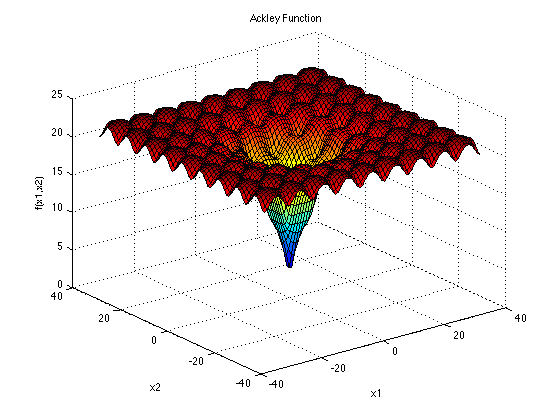
\includegraphics[width=230pt]{ackley.png}
\end{figure}

Esta función fue evaluada (y graficada) con coordenadas de dos dimensiones, en el rango $-32.768 < x_1, x_2 < 32.768$ con los parámetros $a = 20$, $b = 0.2$ y $c = 2\pi$.

La implementación de la fórmula para listas \textit{np.ndarray} de forma ($n$, $d$) puede ser encontrada en el apéndice \ref{app:ackley}.

\subsection{Representación de los individuos}
Las partículas fueron representadas por listas \textit{np.ndarray} de dos elementos, y concatenadas verticalmente, para formar una sola lista de forma ($n$, 2), en donde $n$ es el número de partículas en el enjambre (por defecto 500).

\subsection{Algoritmo de optimización de enjambre de partículas}
El algoritmo descrito en esta tarea fue implementado en dentro de una clase \texttt{ParticleSwarmOptimization}, con dos funciones principales: el constructor y la función \texttt{run}, descritas a continuación.

La implementación del algoritmo puede ser encontrada el apéndice \ref{app:pso}.

\subsubsection{Constructor de la clase \texttt{ParticleSwarmOptimization}}\hfill\\
La primera función sólo sirve para inicializar los argumentos del algoritmo, como son la función de evaluación, el rango de evaluación, el número de partículas y de iteraciones, $\alpha$, $\beta$, la rapidez máxima y una semilla para el generador de números aleatorios.

\subsubsection{Función \texttt{run} de la clase \texttt{ParticleSwarmOptimization}}\hfill\\
En esta función se encuentra el algoritmo en sí, y comienza generando las posiciones de las partículas al azar, guardando una copia de estas como mejores locales, e inicializando la velocidad de las partículas en 0.

Después, por cada iteración del algoritmo:
\begin{enumerate}
  \item Evalúa las partículas usando la función proveída en el constructor (en nuestro caso la función Ackley)
  \item Actualiza la partícula con mejor evaluación global
  \item Actualiza las partículas locales mejores, comparando la evaluación de las partículas locales mejores con la evaluación de las partículas actuales
  \item Actualiza la velocidad de las partículas utilizando $\alpha$, $\beta$, dos coordenadas aleatorias ($\epsilon_1$ y $\epsilon_2$), y los mejores globales ($g^*$) y locales ($x^*$) en la siguiente fórmula
  $$v_{t+1} = v_t + \alpha \epsilon_1 (g^* - x_t) + \beta \epsilon_2 (x^* - x_t)$$
  \item Reduce las velocidades cuya magnitud superan la rapidez máxima
  \item Actualiza las posiciones de las partículas
  $$x_{t+1} = x_t + v_{t+1}$$
\end{enumerate}

Finalmente, la función regresa el historial de la posición de la partícula que tuvo mejor evaluación en cada iteración para poder visualizar el comportamiento del algoritmo.

\section{Resultados}
Para esta demostración se usaron los parámetros por defecto de la clase:
\begin{itemize}
  \item número de partículas = 500
  \item número de iteraciones = 100
  \item $\alpha$ = 2
  \item $\beta$ = 2
  \item $v_{max}$ (rapidez máxima) = 2
\end{itemize}

El único parámetro que se especifica además de la función de evaluación y el rango es \texttt{seed}, inicializado como 0 para que el experimento sea reproducible.

El tiempo total de ejecución es de 2.17 segundos, con la mejor partícula de todas las iteraciones en la posición (0.008138, -0.001466), con una evaluación de 0.025207, encontrada en la iteración 67.

La siguiente gráfica muestra la posición de la mejor partícula en cada evaluación, representando las primeras iteraciones con puntos azules y las últimas con puntos rojos.

\begin{figure}[H]
  \centering
  \includegraphics[width=200pt]{pso_particle.png}
\end{figure}

Se puede observar la similaridad de esta gráfica con la gráfica de la función Ackley en el mismo rango:

\begin{figure}[H]
  \centering
  \includegraphics[width=200pt]{ackley2.png}
\end{figure}

\subsection{Curva de mejor encontrado}
También se incluye una gráfica de la mejor evaluación encontrada por cada iteración. El eje $y$ se graficó en una escala logarítmica para apreciar la mejora muy acelerada en las primeras iteraciones, y después de la iteración 10 mejoras ocasionalmente.

\begin{figure}[H]
  \centering
  \includegraphics[width=\linewidth]{pso_evaluation.png}
\end{figure}

Las mejores evaluaciones se presentan como puntos azules, y además la línea verde muestra el mejor encontrado a través de todas las iteraciones.

\section{Conclusiones y retos encontrados}
En esta práctica se demostró la utilidad y la implementación de uno de los algoritmos cuya creación fue relativamente reciente, además de cómo se comporta cuando las partículas se acercan cada vez más al punto óptimo de la función. Considero que este tipo de algoritmos tienen un muy buen uso para optimización de funciones pero me hubiera gustado profundizar más en las diferentes formas de determinar cuándo parar el algoritmo en vez de sólo usar un número predefinido de iteraciones. 

El reto principal de la implementación pienso que fue diseñar las gráficas en tres dimensiones y crear una implementación con buen desempeño para seleccionar y actualizar los mejores puntos locales en cada iteración.


\bibliographystyle{ACM-Reference-Format}
\bibliography{references}

\clearpage

\appendix

\begin{figure*}
  \section{Implementación de la función Ackley para vectores \textit{np.ndarray}}
  \label{app:ackley}
  \inputminted{python}{/home/mario/git/MarioJim/ITC-Tec/Sem7/InteligenciaComp/EnjambreParticulas/ackley.py}
\end{figure*}

\begin{figure*}
  \section{Implementación del algoritmo de enjambre de partículas}
  \label{app:pso}
  \inputminted[lastline=54]{python}{/home/mario/git/MarioJim/ITC-Tec/Sem7/InteligenciaComp/EnjambreParticulas/particle_swarm.py}
\end{figure*}

\begin{figure*}
  \inputminted[firstline=56]{python}{/home/mario/git/MarioJim/ITC-Tec/Sem7/InteligenciaComp/EnjambreParticulas/particle_swarm.py}
\end{figure*}

\end{document}
\endinput